En BJT består av 3 deler: collector, base og emittor.
Disse er bygget opp av tre dopede halvleder materialer, n-type og p-type.
Mellom disse regionene er pn-overganger akkurat som i dioder. \\\\
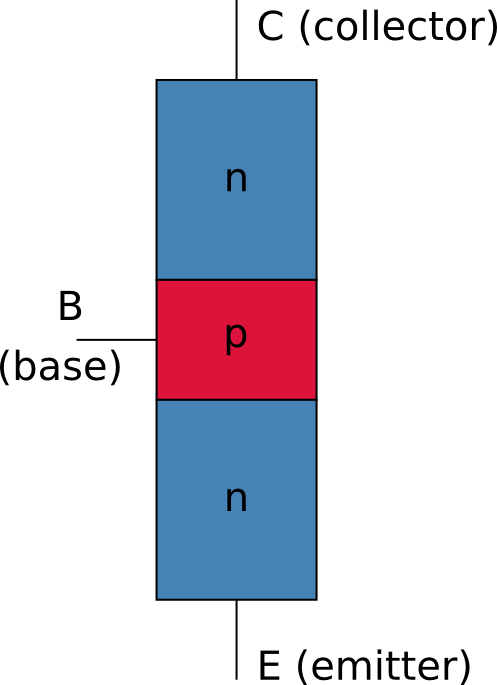
\includegraphics[width=0.5\textwidth]{./img/npn}
\\\\
Symbolet for BJTer ser slik ut for npn \\\\
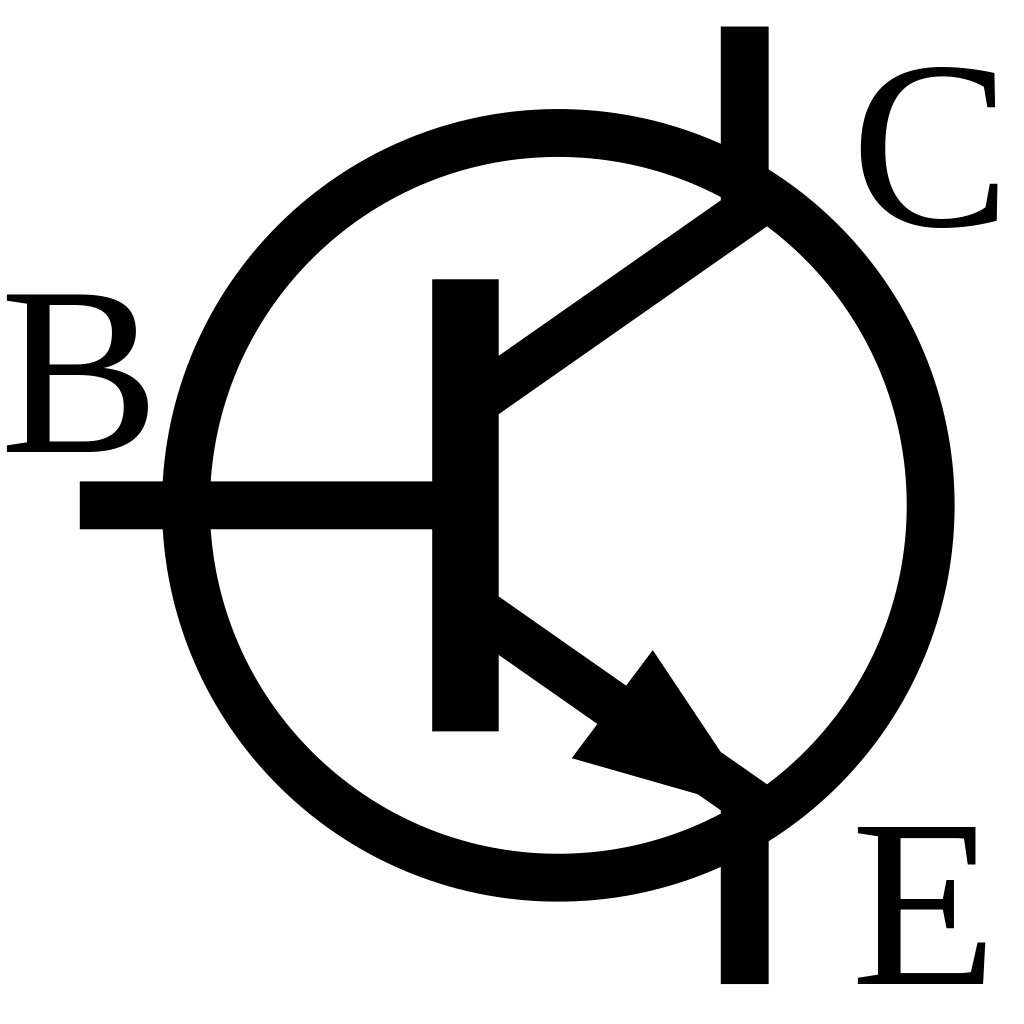
\includegraphics[width=0.25\textwidth]{./img/npn-symbol} \\
Hvor den lille pilen peker mot det n-dopede materialet.
\\
Tilsvarende for pnp \\\\
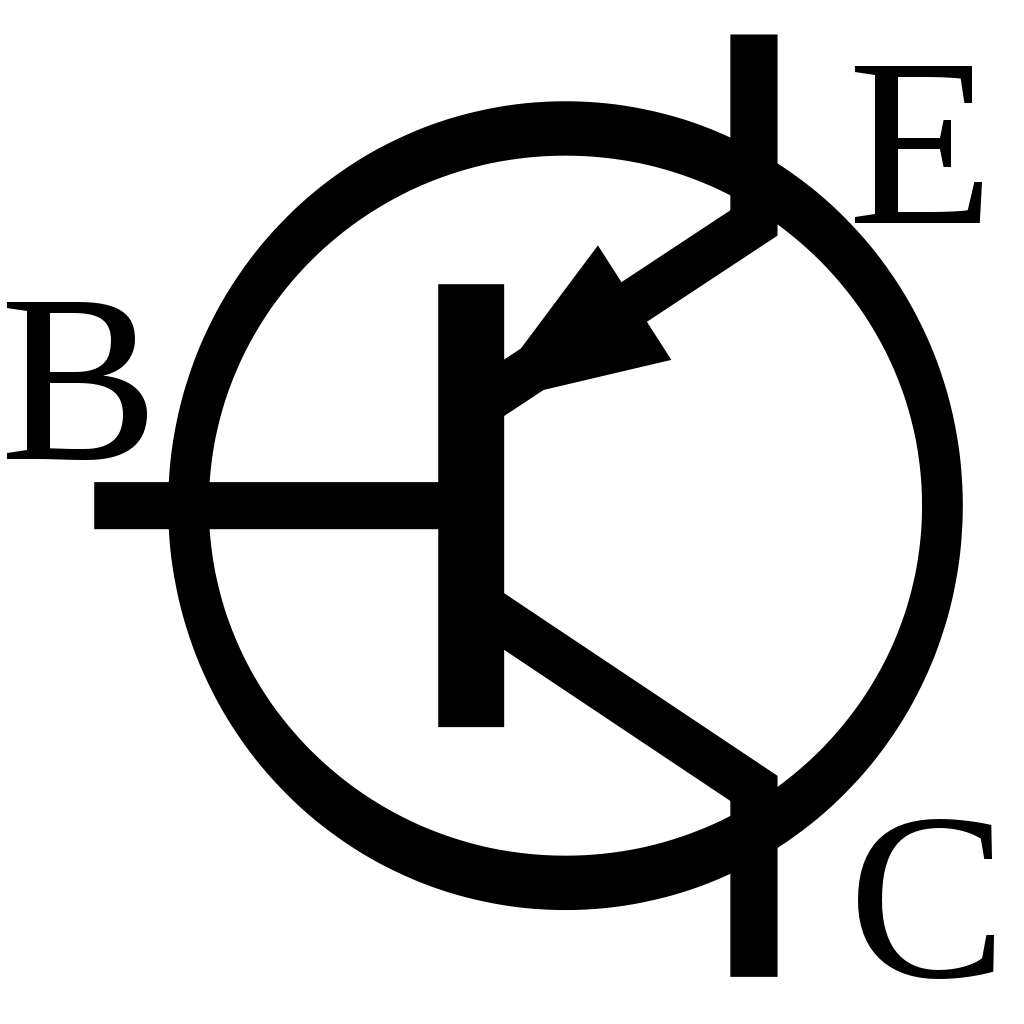
\includegraphics[width=0.25\textwidth]{./img/pnp-symbol}
